\section{Aplicações Práticas de Árvores}

\begin{frame}[plain]
  \centering
  \Huge \insertsection
\end{frame}

% --- Árvore Genealógica ---
\begin{frame}{Árvore Genealógica}
  \begin{itemize}
    \item Uma aplicação clássica de árvores é na representação de relações familiares.
    \item Cada \textbf{nó} representa uma pessoa, e cada \textbf{aresta} representa uma relação de parentesco.
    \item A raiz representa um ancestral comum, e os descendentes são dispostos em níveis inferiores.
    \item Quanto mais alto o nó na árvore, mais descendentes ele pode ter.
  \end{itemize}
\end{frame}

\begin{frame}{Árvore Genealógica}
    \centering  
    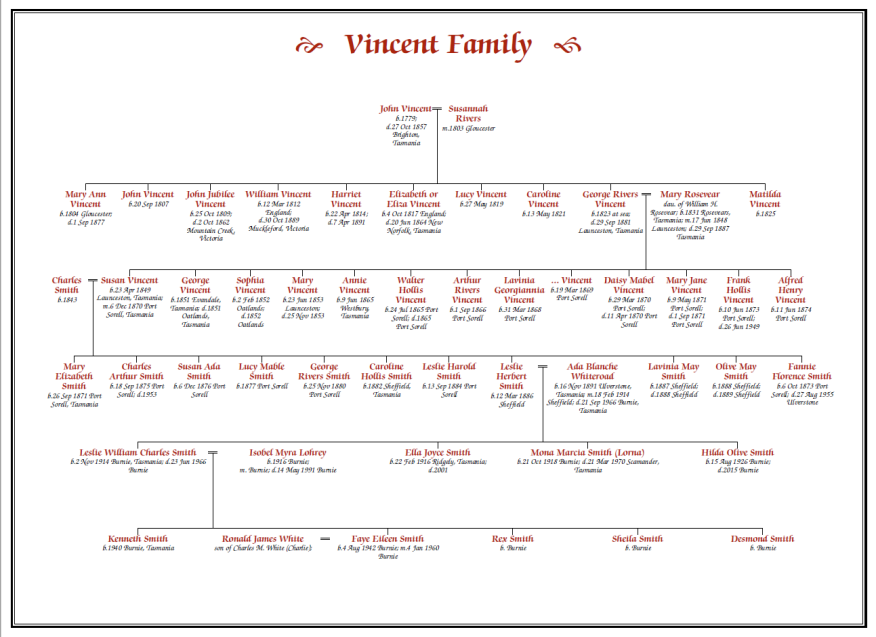
\includegraphics[width=1\textwidth]{./images/famtree.png}
\end{frame}

% --- Expressões Matemáticas ---
\begin{frame}{Árvores de Expressão Matemática}
  \begin{itemize}
    \item Expressões matemáticas podem ser representadas em forma de árvore binária.
    \item Cada operador (\texttt{+}, \texttt{-}, \texttt{*}, \texttt{/}) ocupa um nó interno.
    \item Cada número ou valor constante ocupa uma folha.
    \item Essa estrutura ajuda o computador a \textbf{definir a ordem correta das operações} (ordem de precedência).
  \end{itemize}
\end{frame}

\begin{frame}{Exemplo de Árvore de Expressão}
  \centering
  
  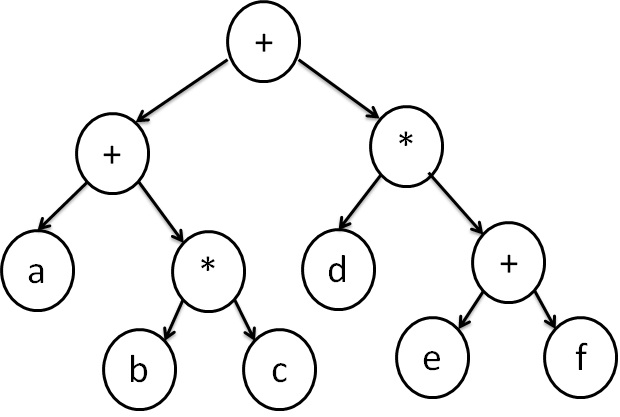
\includegraphics[width=0.8\textwidth]{./images/exp.jpg}
  
  \vspace{0.3cm}
  
  \textit{Exemplo: Representação da expressão \((a + b * c) + (d * (e + f))\)}
\end{frame}

% --- Percursos em Árvores ---
\begin{frame}{Percursos em Árvores (Traversals)}
  \begin{itemize}
    \item Formas diferentes de visitar os nós:
    \item \textbf{Pré-fixa (pré-ordem):} visita a raiz, depois o filho esquerdo e direito.
    \item \textbf{In-fixa (ordem simétrica):} visita o filho esquerdo, a raiz e o direito.
    \item \textbf{Pós-fixa (pós-ordem):} visita o filho esquerdo, depois o direito e por fim a raiz.
  \end{itemize}
\end{frame}

\begin{frame}{Comparação dos Percursos}
  \centering
  \begin{tabular}{|c|l|}
    \hline
    \textbf{Tipo} & \textbf{Ordem de Visita} \\
    \hline
    Pré-fixa & Raiz → Esquerda → Direita \\
    In-fixa & Esquerda → Raiz → Direita \\
    Pós-fixa & Esquerda → Direita → Raiz \\
    \hline
  \end{tabular}
  \vspace{0.5cm}


  \textit{Cada percurso gera uma forma diferente de ler a mesma árvore.}
\end{frame}
